\documentclass[11pt]{article}
\usepackage[margin=1in]{geometry}
\usepackage{amsmath,amssymb,amsthm}
\usepackage{graphicx}
\usepackage{float}
\usepackage[T1]{fontenc}
\usepackage{lmodern}
\usepackage{microtype}
\usepackage[hidelinks]{hyperref}

\newtheorem{lemma}{Lemma}
\newtheorem{theorem}{Theorem}
\newcommand{\MA}{M\!A}
\newcommand{\Cb}{C_{\mathrm b}}
\newcommand{\norm}[1]{\lVert #1\rVert}

\title{The Fourier-Multiplier Induction Map\\
Is Not Well Defined in General}
\author{Full solution packet for arXiv:2011.00146}
\date{22 July 2026}

\begin{document}
\maketitle

\begin{center}
\fbox{\parbox{0.89\textwidth}{\textbf{Status: full solution likely valid.}
For every uniform lattice $\Gamma<\mathrm{SL}(3,\mathbb R)$ covered by the
source theorem, some $m\in\MA(\Gamma)$ has induced function
$\widehat m\notin\MA(\mathrm{SL}(3,\mathbb R))$.}}
\end{center}

\section{Source question and context}

Battseren considers a lattice $\Gamma$ in a locally compact group $G$, a
normalized Borel fundamental domain $\Omega$, and the induction formula
\begin{equation}\label{eq:induction}
 \Phi:\ell^\infty(\Gamma)\longrightarrow\Cb(G),\qquad
 \Phi(m)(x)=\widehat m(x)
 =\int_\Omega m(\gamma(x\omega))\,d\omega.
\end{equation}
Here $\gamma:G\to\Gamma$ is determined by the decomposition
$G=\bigsqcup_{y\in\Gamma}\Omega y$.  Lemma 18 of the arXiv version proves
that \eqref{eq:induction} is well defined and that it restricts contractively
to the Fourier algebra and the completely bounded multiplier algebra
\cite{Battseren}.  For a uniform lattice $\Gamma$ in
$G=\mathrm{SL}(3,\mathbb R)$, Theorem A proves that it does not give a bounded
map $\MA(\Gamma)\to\MA(G)$.

Immediately after that proof, the source asks in Remark 19:
\begin{quote}
``We do not know if the map $\Phi:\MA(\Gamma)\to\MA(G)$ is well defined.''
\end{quote}
The 2024 journal version retains the same question as Remark 4.2 and labels
the unboundedness statement Theorem B.

\begin{figure}[H]
 \centering
 
\includegraphics[width=0.96\textwidth]{figures/open_problem_crop.png}
 \caption{Remark 19 in the original arXiv paper, PDF page 10.}
\end{figure}

\section{Proof intuition}

The source already supplies the hard harmonic analysis: boundedness of a
hypothetical restriction is impossible.  The missing step is purely
functional analytic.  Formula \eqref{eq:induction} is continuous in the
ambient sup norms, while each Fourier multiplier norm is stronger than the
sup norm.  Therefore, if the restriction were defined on every multiplier,
any multiplier-norm convergent graph sequence would have the same uniform
limit on both sides.  Its graph would be closed, and the closed graph theorem
would force boundedness---exactly what the source theorem excludes.

\section{The closed-graph lemma}

\begin{lemma}\label{lem:sup}
For every locally compact group $H$ and every $m\in\MA(H)$,
\[
 \norm{m}_\infty\leq\norm{m}_{\MA(H)}.
\]
\end{lemma}

\begin{proof}
Fix $x\in H$.  Choose a unit vector $\xi\in L^2(H)$ and define the coefficient
function
\[
 u(y)=\langle\lambda(y)\xi,\lambda(x)\xi\rangle.
\]
Then $u\in A(H)$, $u(x)=1$, and $\norm{u}_{A(H)}\leq1$.  Since the Fourier
algebra norm dominates the sup norm,
\[
 |m(x)|=|(mu)(x)|\leq\norm{mu}_{A(H)}
 \leq\norm{m}_{\MA(H)}\norm{u}_{A(H)}
 \leq\norm{m}_{\MA(H)}.
\]
Take the supremum over $x$.
\end{proof}

\begin{lemma}\label{lem:closed}
Let $\Gamma<G$ be a lattice and let $\Phi$ be given by
\eqref{eq:induction}.  If
\[
 \Phi(\MA(\Gamma))\subseteq\MA(G),
\]
then the restriction $\Phi:\MA(\Gamma)\to\MA(G)$ is bounded.
\end{lemma}

\begin{proof}
The normalized integral formula gives the ambient contraction
\begin{equation}\label{eq:ambient}
 \norm{\Phi(m)}_\infty\leq\norm{m}_\infty
 \qquad(m\in\ell^\infty(\Gamma)).
\end{equation}
Suppose $m_n\to m$ in $\MA(\Gamma)$ and
$\Phi(m_n)\to h$ in $\MA(G)$.  By Lemma~\ref{lem:sup}, both convergences imply
uniform convergence.  Equation \eqref{eq:ambient} also gives
\[
 \Phi(m_n)\longrightarrow\Phi(m)
 \quad\text{uniformly on }G.
\]
Uniqueness of uniform limits yields $h=\Phi(m)$.  Hence the graph of the
restriction is closed.  Both multiplier spaces are Banach spaces, so the
closed graph theorem \cite[Theorem 2.15]{Rudin} makes the restriction bounded.
\end{proof}

\section{Full negative answer}

\begin{theorem}\label{thm:main}
Let $\Gamma$ be a uniform lattice in $G=\mathrm{SL}(3,\mathbb R)$ and let
$\Phi$ be the induction formula used in \cite{Battseren}.  Then
\[
 \Phi(\MA(\Gamma))\not\subseteq\MA(G).
\]
Equivalently, there exists $m\in\MA(\Gamma)$ for which the induced bounded
continuous function $\widehat m=\Phi(m)$ is not a Fourier multiplier of $G$.
\end{theorem}

\begin{proof}
Assume instead that $\Phi(\MA(\Gamma))\subseteq\MA(G)$.  By
Lemma~\ref{lem:closed}, the restriction
$\Phi:\MA(\Gamma)\to\MA(G)$ is bounded.  This contradicts Theorem A of the
arXiv source (Theorem B of the published version), which proves that the same
restriction cannot be bounded for such a uniform lattice.  Therefore the
restriction is not everywhere well defined.
\end{proof}

\section{Verification, novelty, and limitations}

The proof has no numerical or finite-search dependency.  Its four interfaces
are explicit: the source integral formula gives \eqref{eq:ambient};
Lemma~\ref{lem:sup} gives both continuous embeddings into sup norm; uniqueness
of uniform limits closes the graph; and the source theorem supplies the
unboundedness contradiction.  The published proof itself begins by assuming
that the restriction is ``well defined and bounded,'' so the quantifiers match
the contradiction used here.

A bounded novelty search on 22 July 2026 covered the run's four cheap indexes;
the exact arXiv id, title, author, and well-definedness phrase; arXiv searches
combining $\MA(\Gamma)$, $\MA(G)$, induction, well defined, and closed graph;
the open-access 2024 journal version; and the author's later arXiv:2408.09638 on
$M_d$ multipliers and lattices.  No later resolution or occurrence of this
closed-graph argument was found.

Novelty confidence is moderate because the argument is elementary and may be
folklore or implicit in the published theorem's wording.  The explicit Remark
4.2 nevertheless remains in the published paper.  The theorem here is limited
to the induction formula and the uniform $\mathrm{SL}(3,\mathbb R)$ lattices
covered by the source unboundedness theorem; it does not classify other
lattice pairs and does not resolve the paper's amenability conjecture.

Human review should focus on the interpretation and quantifiers of the source
unboundedness theorem.  Once those are accepted, the closed-graph step is
complete.

\begin{thebibliography}{9}
\bibitem{Battseren}
B.-O. Battseren,
\emph{On the growth of Fourier multipliers},
arXiv:2011.00146; J. Noncommut. Geom. 18 (2024), no.~4, 1209--1228,
\url{https://doi.org/10.4171/JNCG/551}.

\bibitem{Rudin}
W. Rudin,
\emph{Functional Analysis}, second edition,
McGraw--Hill, 1991.
\end{thebibliography}

\section*{Source evidence}

\begin{figure}[H]
 \centering
 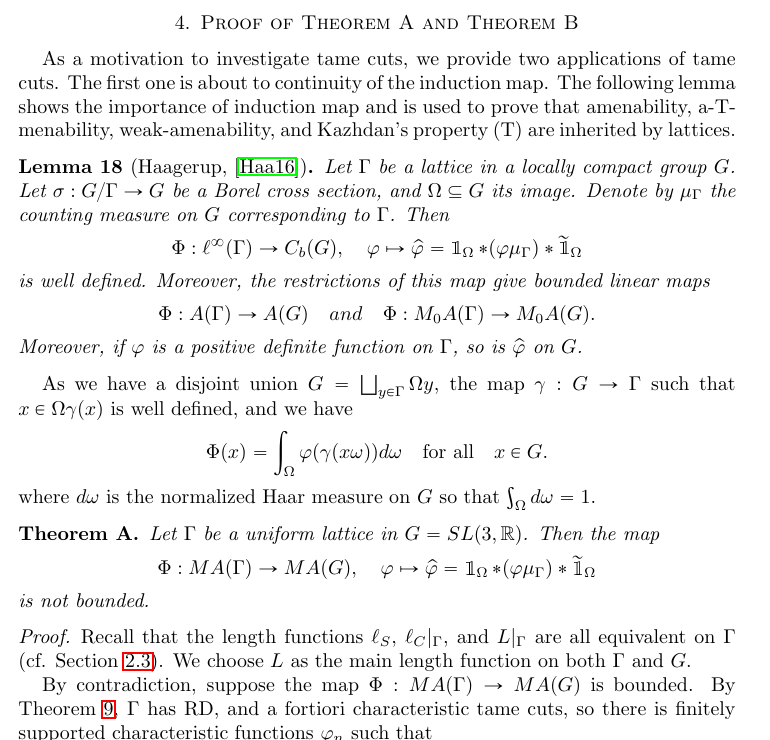
\includegraphics[width=0.66\textwidth]{figures/induction_and_unboundedness_crop.png}
 \caption{The induction formula and source Theorem A, arXiv PDF page 9.}
\end{figure}

\end{document}
